\RequirePackage[l2tabu, orthodox]{nag}

\documentclass[11pt]{article}

\usepackage{amsmath}    			% ams packages for mathematics environment    
\usepackage{amssymb}
\usepackage{amsfonts}
\usepackage{amsthm}

\usepackage{graphicx}  				% Versatile graphics manipulation options

\usepackage[croatian]{babel}  % Croatian typographical rules and hyphenation patterns 
\usepackage[utf8]{inputenc}  	% Encoding of Croatian characters
\usepackage[T1]{fontenc}
\usepackage{ae,aecompl}     	% Type 1 fonts, similar to Computer Modern

\usepackage{microtype}				% Improves spacing

\usepackage{booktabs}					% Nice looking tables
\usepackage{enumerate}				% Additional options for listing of items in enumerate environment
\usepackage{algorithm2e}			% Writing pseudo-code
\usepackage{todonotes}				% Adding todo items
\usepackage{dirtree}					% Simple display of directory tree
\usepackage{hyperref}					% Managing cross-referencing

\graphicspath{{./figures/}}

\newcommand { \sqmatrix }[5]{
	\ensuremath {
	#1=\begin{bmatrix}
			#2 & #3 \\
			#4 & #5 
		\end{bmatrix}
	}
}

\begin{document}

\title{Larics Latex Coding Standard}
\author{Vrijedni Laricsovac}
\maketitle
%\tableofcontents

%\begin{abstract}
%		In this document we give recommendations on how to structure and prepare your Latex project.  
%\end{abstract}

\section{Structure and formatting}
\label{sec:structure}
 
Recommended structure of your Latex project is as follows: 

\dirtree{%
.1 main folder.
	.2 content. 
		.3 {chapter1.tex}.
		.3 {chapter2.tex}.
	.2 figures.
		.3 source.
			.4 {experiment1.vsd}.
		.3 {experiment1.pdf}.
	.2 bibliography.
		.3 {mybibliography.bib}.
	.2 {main.tex}. 
}

Format the text according to WYSIWYG (What You See Is What You Get) rule - separate paragraphs with a blank line; indent items in tabulated environments.

When uploading your project to a version control repository, upload only files which are necessary to 
generate the desired output file. 

\section{Labeling}
\label{sec:labeling}

Labels should have indicative prefixes - fig for Figures, sec for Sections, tab for Tables, eq for equations. Two labeling examples are given, for Figure \ref{fig:shapes} and for Table \ref{tab:experiment1_data}. To ensure quality, always use vector graphic images. 

\begin{figure}[ht!]
	\centering
		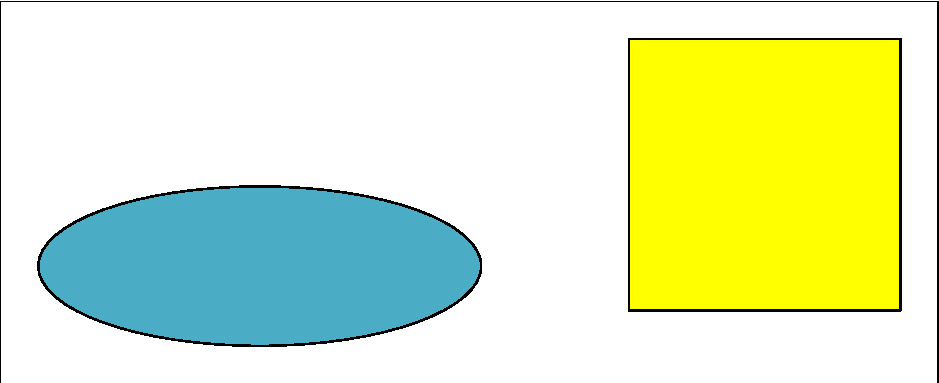
\includegraphics[width=0.7\linewidth]{shapes.pdf}
	\caption{Figure explanation goes here}
	\label{fig:shapes}
\end{figure}

\begin{table}[ht!]
	\centering
	\begin{tabular}{ccc}
		\toprule
		Station & $t_e [h]$ & $c_e^2$ \\
		\midrule
		1       & 1.5       & 1.5\\
		2       & 1.6       & 0.75\\
		\bottomrule
	\end{tabular}
	\caption{Table data description goes here}
	\label{tab:experiment1_data}
\end{table}

Bibitems should be labeled according to the first author surname and publication date, for example 'sewlal2014'. Useful resources on the topic of best practices in LaTeX are, for example, \cite{sewlal2014} and \cite{birotic2015}.



\section{Useful Packages}
\label{sec:packages}

Here is a list of useful packages:
\begin{itemize}
	\item{nag}
	
	This package checks for obsolete LaTeX packages and outdated commands. Package needs to be loaded in the first lines of your preamble, before the documentclass command.
	
	\item{amsmath, amsthm, amssymb, amsfonts}
	
	Standard packages for math environments. Compared to other similar packages, they have some advantages, such as more versatile alignment options. Nice intro to amsmath can be found \href{https://www.sharelatex.com/learn/Aligning_equations_with_amsmath}{here}.
		
	\item{graphicsx}
	
	Package needed for embedding figures. Using command graphicspath we can set the path to one or more folders that contain figures. 
			
	\item{hyperref}
	
	This package provides useful commands for inserting links pointing inside or outside the document. When included, it automatically turns all your internal references into hyperlinks. Package info can me found \href{https://en.wikibooks.org/wiki/LaTeX/Hyperlinks}{here}.
	
	\item{booktabs}
	
	This package is used to create nicer tables than provided by Latex by default. Table \ref{tab:experiment1_data} is written using booktabs package. Package info can be found \href{http://ctan.ijs.si/tex-archive/macros/latex/contrib/booktabs/booktabs.pdf}{here}.  Package csvsimple is used for importing csv format tables.
	
	\item{geometry}
	
	This package is an easy interface for modification on page dimensions and margins. However, size customization is not advisable, and should be used only when necessary.
	
	\item{todonotes}
	
	The todonotes package allows you to insert to do items in your document.
	
	
	\item{algorithm2e}
	
	Algorithm2e is an environment for writing algorithms, where an algorithm behaves as a floating object. Algorithm \ref{alg:multiplication} is written using algorithm2e package.
	
	\begin{algorithm}[h]
		\label{alg:multiplication}
    \KwData{$n$}
    \KwResult{$n^{10}$}
    $res = n; i=1$\;
    \While{$i < 10$}{
		    $i++$\;
        $res = res *n$\;
    }
		\Return $res$;
		\caption{Basic algorithm}
	\end{algorithm}
	
	\item{microtype}
	 
	This package improves the spacing between words and letters. Load this package after fonts packages.
	
\end{itemize}

Sometimes it is useful to define our custom commands, when certain parts repeat throughout the text. Here is an example of usage of a user-defined command: \sqmatrix{A}{3}{4}{5}{6} and  \sqmatrix{B}{7}{8}{9}{10}.


\appendix
\chapter{Appendix}

Ovdje ide appendix.


\bibliographystyle{ieeetr}
\bibliography{bibliography/my_bibliography}

\end{document}
